
\documentclass[11pt, letterpaper]{article}

% PAGE LAYOUT
\usepackage{geometry} 
\geometry{letterpaper, left=1.25in, right=1.0in, top=1.0in, bottom=1.0in}

% FONT 
\usepackage{graphicx}
\usepackage{fontspec} 
\usepackage[usenames,dvipsnames]{xcolor}
\usepackage{xunicode}
\usepackage{xltxtra}
\defaultfontfeatures{Mapping=tex-text}
\usepackage{lmodern}
\renewcommand*{\familydefault}{\sfdefault}
\usepackage{dashrule}

% PDF PROPERTIES
\usepackage[%dvipdfm, 
bookmarks, colorlinks, breaklinks, 
pdftitle={Reactive Motor Manual},
pdfauthor={Caitrin Eaton},
%pdfproducer={http://uci.edu\~azizi}
]{hyperref}  
\hypersetup{linkcolor=blue,citecolor=blue,filecolor=black,urlcolor=cyan!85!magenta} 

% TITLE
\title{Reactive Motor Controller Manual}
\author{Caitrin Eaton}
\date{December 5, 2016}

% DOCUMENT
\begin{document}
	
\maketitle

\tableofcontents

\newpage
\part{User's Guide}
\section{What the Reactive Motor Controller does}
\label{sec:overview}
The Reactive Motor Controller is designed to interface with the Aurora Scientific suite of voltage-controlled motors. It accepts an input voltage that is assumed to represent the current state of the motor (usually \texttt{FORCE OUT}), and generates an output voltage that can be used to command the next state of the motor (usually \texttt{LENGTH IN}). The overall effect is that of a voltage spring: $V_{out} = k_{V}*V_{in}$, where $V_{in}$ is the voltage that is read in and  $V_{out}$ is the generated output voltage. When $V_{in}$ is tied to \texttt{FORCE OUT}, and $V_{out}$ to \texttt{LENGTH IN}, the position of the Aurora Scientific motor will be adjusted as a function of force such that it acts as a mechanical spring. The spring constant is defined in software and can be adjusted between trials.



\section{Requirements for use}
\label{sec:requirements}

\subsection{Voltage source}
Once programmed, the Reactive Motor Controller requires a voltage source with +15~V, -15~V, +5~V, and GND outputs. The current draw is relatively low (10-20~mA), and a source rated at 0.25 W power should be more than adequate. 

\subsection{Computer with powered USB}
A computer running Linux or Windows is required in order to program the BeagleBone and to send commands to be executed on the BeagleBone. This communication happens over powered USB. If the USB port is not powered, the BeagleBone will still draw enough current to turn on and light up, but will not properly support communication, command execution, or digital I/O. When multiple powered USB ports are available, not all are guaranteed to work. The logic behind this is unclear to your humble author. But, if the BeagleBone seems unresponsive even after drivers have been installed, or attempts to establish an SSH connection repeatedly result in errors, then try plugging the BeagleBone into other powered USB ports on the same machine. So far, our lab has not had any problems that could not be solved by a USB round-robin or driver installation.

\subsection{Data acquisition}
The provided software does not log data on the BeagleBone, so an external data acquisition (DAQ) system, e.g. one of National Instrument's NI DAQ systems, can be used to monitor \texttt{LENGTH IN} and \texttt{FORCE OUT} voltage signals. These can then be visualized and recorded on your computer with a data analysis program like Igor, LabView, or MATLAB.
	
	
	
\section{Installing BeagleBone drivers on a new computer}
\label{sec:drivers}
If the computer has never been connected to a BeagleBone before, you may have to install some drivers. Instructions are included below.  \textit{Note: If you're using Linux, no drivers need to be installed.}
\begin{enumerate}
	\item Connect the BeagleBone via \emph{powered} USB to a computer with an Internet connection. 
	\item Open a file browser window and navigate to the BeagleBone folder, which will appear as an external drive, similar to a USB memory stick.
	\item Right click \texttt{START.htm} and select \texttt{Open with Chrome}. (Internet Explorer will not work.)
	\item In the page that opens, there should be three clearly marked installation steps on the left side. 
	\item \texttt{Step 1: Plug in BeagleBone via USB} should be highlighted in green with a check mark. If not, the BeagleBone may not be connected to a powered USB.
	\item Left click \texttt{Step 2: Install drivers} and follow the instructions in the provided table as appropriate for your operating system. These drivers let your computer talk to the BeagleBone.  If installation is unsuccessful, the BeagleBone may not be connected to a powered USB.
	\item After installing drivers, restart your computer.
	\item Re-open \texttt{START.htm} in Chrome.  \texttt{Step 2: Install drivers} should be highlighted in green with a check mark.
	\item \texttt{Step 3: Browse to web server on board} is unnecessary. There are some interactive scripts there that are helpful if you'd like to learn about general BeagleBone programming, but that's not necessary in order to use the Reactive Motor Controller or edit the spring constant.
\end{enumerate}

You can now program the BeagleBone from this computer by establishing an SSH connection.


\section{Establishing an SSH connection}
\label{sec:ssh}
An SSH connection makes it possible to program and control the BeagleBone Black from any computer with the proper drivers (see Section~\ref{sec:drivers}), similar to working in a Remote Desktop environment. 

\subsection{On Linux}
To establish an SSH connection from a Linux terminal:
 
 \begin{enumerate}
 	\item Connect the BeagleBone via \emph{powered} USB to a computer with drivers already installed. 
 	\item Open a terminal window.
 	\item Enter into the terminal: \texttt{sudo ssh 192.168.7.2 -l root}
 	\item You will probably be prompted to enter the computer's password. This is the regular password for your computer. For what I assume are paranoid Linux-hacker security reasons, no characters will appear as you type. Simply enter your password as usual and then hit \texttt{ENTER}.
 	\item If SSH does not succeed, the BeagleBone may not be connected to a powered USB.
 	\item If SSH succeeded, the terminal is now running on the BeagleBone, rather than your computer. Any commands you enter will be executed on the BeagleBone. For starters, list the contents of the current folder with the command \texttt{ls}.
 \end{enumerate}
 
\subsection{On Windows}
To establish an SSH connection from PuTTY on a Windows machine:

\begin{enumerate}
	\item Make sure PuTTY is installed. If not, download it for free from \href{wwww.putty.org}{www.putty.org}. 
	\item Open PuTTY.
	\item In the IP field, enter: \texttt{192.168.7.2}
	\item Make sure the \texttt{SSH} option is selected. (I believe the default is Telnet, which will not work here.)
	\item A terminal window will open, connected to the BeagleBone. When it gives you the login prompt, type \texttt{root} and hit \texttt{ENTER}.
	\item If the window does not appear or gives you an error message instead of a login prompt, the BeagleBone may not be connected to a powered USB.
	\item If SSH succeeded and you have logged in as \texttt{root}, the terminal is now running on the BeagleBone, rather than your computer. Any commands you enter will be executed on the BeagleBone. For starters, list the contents of the current folder with the command \texttt{ls}.
\end{enumerate}

\subsection{CAUTION: Safely disconnecting the BeagleBone}

When you are done, it is important to enter the command \texttt{poweroff}, so that the BeagleBone shuts itself down before it is unplugged from the powered USB port. Once all the lights have gone off, it is safe to close the terminal window and unplug the BeagleBone.



\section{Programming the BeagleBone}
\label{sec:prog}
The BeagleBone can be programmed from an external computer through a terminal window in which an SSH connection has been established. This must be the same terminal window in which you have logged in to the BeagleBone. Should you accidentally close this terminal window, re-connect by following the steps in Section~\ref{sec:ssh}. Remember that the terminal is running on the BeagleBone, which has a Debian Linux operating system. If you're feeling stuck at any point using the terminal, it might be helpful to do an online search for Debian commands. The provided code is written in C++, which is also very well documented with free online educational resources.

The Reactive Motor Controller software is assumed here to have been provided in the file \texttt{ReactiveMotor.cpp}. 

\subsection{CAUTION: The Typocalypse}
Be very careful with spelling in all of your interactions with the terminal. Double check all commands for typos before hitting \texttt{ENTER}. The terminal will execute \emph{exactly} the command you enter, regardless of what you may mean to do, sometimes with frustrating results. The terminal has no spellcheck, autocorrect, or common sense. For a modern human, this feels a lot like having your smartphone replaced by a sextant and carrier pigeon. Be vigilant. Thar be dragons.

\subsection{Configuring BeagleBone I/O pins}
The I/O pins on the BeagleBone must be configured before running Reactive Motor Controller code. This is done by loading the included configuration files with the commands
\begin{quote}
	\texttt{echo spi0-loop > \$SLOTS}\\
	\texttt{echo ADAFRUIT-SPI0 > \$SLOTS}
\end{quote}
where the 0s in \texttt{spi0-loop} and {ADAFRUIT-SPI0} are zeros, not letter Os. The O in \texttt{\$SLOTS} is the capital letter O, not a zero. The order of these commands is also very important. Load \texttt{spi0-loop} first, {ADAFRUIT-SPI0} second.

Pin configuration only needs to be done once after the BeagleBone starts up. Code can then be executed as many times as you like without reconfiguring the pins again until the next time the BeagleBone starts up.

\subsection{Backing up code}
It is a good idea to copy this code into a new file before editing, so that you always have a backup. 
In order to copy the original file \texttt{ReactiveMotor.cpp} into a new file named \texttt{ReactiveMotor\_Backup.cpp}, enter:
\begin{quote}
	\texttt{cp ReactiveMotor.cpp ReactiveMotor\_Backup.cpp}
\end{quote}
For more information on file handling in Debian, e.g. how to create and copy into different folders, do an online search for \emph{Debian terminal file handling}.

In order to restore your code from the backed-up copy, use the same \texttt{cp} command:
\begin{quote}
	\texttt{cp ReactiveMotor\_Backup.cpp ReactiveMotor.cpp}
\end{quote}
You may want to give your new code file a distinctive name in the place of \texttt{ReactiveMotor.cpp}. Feel free to put any name here, as long as it ends with the extension \texttt{.cpp}. 

\subsection{Editing and compiling code}
To edit code, open it in the text editor ``nano'' using the command
\begin{quote}
	\texttt{nano ReactiveMotor.cpp}
\end{quote}
where you can replace \texttt{ReactiveMotor.cpp} with the name of any existing file you would like to edit. Be forewarned that if you misspell the file name, nano will create a new (empty) file with the name that matches your command, and the editor will open with an empty screen. Return to the command line (regular terminal) by exiting nano with the command \texttt{CTRL+x} and try again.

With your code open in nano, be aware of nano's custom commands, which listed at the bottom of the terminal window. In this list, the caret symbol \texttt{$^\wedge$} is used to represent the control button \texttt{CTRL}. The most useful of these commands are:
\begin{itemize}
	\item Save is \texttt{CTRL+o} (written \texttt{$^\wedge$o} in the nano command list)
	\item Exit (return to the command line) is \texttt{CTRL+x} (written \texttt{$^\wedge$x} in the nano command list)
	\item Scrolling and cursor movements are done with arrow buttons, not with the mouse.
	\item Copy and paste are done with the mouse's right-click menu. Windows shortcuts like \texttt{CTRL+c} and \texttt{CTRL+v} will not work.
\end{itemize}
Note that nano will not save your work automatically on exiting, so you must save with \texttt{CTRL+o} before returning to the command line.

After editing your code, you will have to recompile it. Otherwise the BeagleBone will continue to execute the version of your code that was most recently compiled. To compile the newly edited \texttt{ReactiveMotor.cpp}:
\begin{quote}
	\texttt{g++~~ReactiveMotor.cpp~~GPIO.cpp~~-o~~ReactiveMotor.o~~-pthread}
\end{quote}
If your code file has another name, replace \texttt{ReactiveMotor.cpp} and \texttt{ReactiveMotor.o} with the correct file name. The extensions \texttt{.cpp} and \texttt{.cpp} should stay the same. 

\subsection{Executing code}
In order to run your compiled code, enter
\begin{quote}
	\texttt{./ReactiveMotor.o}
\end{quote}
where \texttt{ReactiveMotor.o} can be replaced by the name of your compiled \texttt{.o} file.
	

\section{Guide to the code}
To do.

\newpage
\part{Fabrication}
This section explains how to fabricate a new Reactive Motor Controller.

\section{Parts}
Parts required to construct and control the custom PCBs are listed here in the format <name: description (quantity)>.

\begin{itemize}
	\item Adafruit BSS138: 4-channel I2C-safe bi-directional logic level converter (2)
	\item ADS7813P: Low-power, serial 16-bit sampling analog-to-digital converter (1)
	\item AD7849CN: Serial input, 14-bit/16-bit digital-to-analog converter (1)
	\item AD588BQ: Multiple output, high precision, dual-tracking reference (1)
	\item 450-650 $\Omega$ resistor: through hole (1)
	\item 39 k$\Omega$ resistor: 1\% tolerance, through hole (1)
	\item 100 k$\Omega$ potentiometer: 10-turn, high precision (2)
	\item 0.01 $\mu$F (10 nF) ceramic capacitor: rated for over 15 V (1)
	\item 0.1 $\mu$F ceramic capacitor: rated for over 15 V (1)
	\item 1 $\mu$F ceramic capacitor: rated for over 15 V (1)
	\item 1 $\mu$F electrolytic capacitor: rated for over 15 V (2)
	\item 10 $\mu$F electrolytic capacitor: rated for over 15 V (1)
	\item 1N4148: Schottky diode (1)
	\item 1N5711: Schottky diode (1)
	\item LED: red (1)
	\item Push button (1)
	\item Ribbon cable: 12- or 14-pin, 6", female/socket (1)
	\item Pin header: 12- or 14-pin, 2-row, female (2)
	\item Pin header: 12- or 14-pin, 2-row, male (2)
	\item Screw terminal: 3-pin, 0.137~in (3.5~mm) spacing (4)
	\item Spacer: 0.5"-1", fits 4-40 screw (8)
	\item 4-40 screw: 0.25"-0.5" (8)
	\item Custom PCB: plans attached (1)
	\item Adafruit BeagleBone Black Proto Cape (1)
	\item Insulated wire: 22 awg (as needed)
\end{itemize}

Also required to interface with BeagleBone and Aurora Scientific control box:
\begin{itemize}
	\item Power source with +15 V, -15 V, +5 V, and GND terminals
	\item Aurora Scientific motor control box with 300-series motor
	\item Independent data acquisition system, e.g. NI DAQ
	\item Computer with powered USB port, used to SSH onto the BeagleBone
	\item So many BNC cables (to connect Aurora with the data acquisition system and custom voltage control PCB, and to connect the power source to the custom voltage control PCB)
\end{itemize}


\section{Circuit design}
The reactive motor circuit is designed to convert an incoming $\pm10$~V force signal from the Aurora Scientific motor control black box into digital values with the ADC chip, and to generate an outgoing $\pm10$~V position control signal with the DAC chip. The PCB design is sketched out in Figure~\ref{figAnnex}

The BeagleBone Black handles ADC readings and DAC commands over an ISP bus. Code running on the BeagleBone Black processes the force reading and computes a desired position command. The custom cape in Figure~\ref{figCape} handles digital communications between the BeagleBone and voltage control PCB (Figure~\ref{figAnnex}).



\begin{figure}[!p]
	\centering
	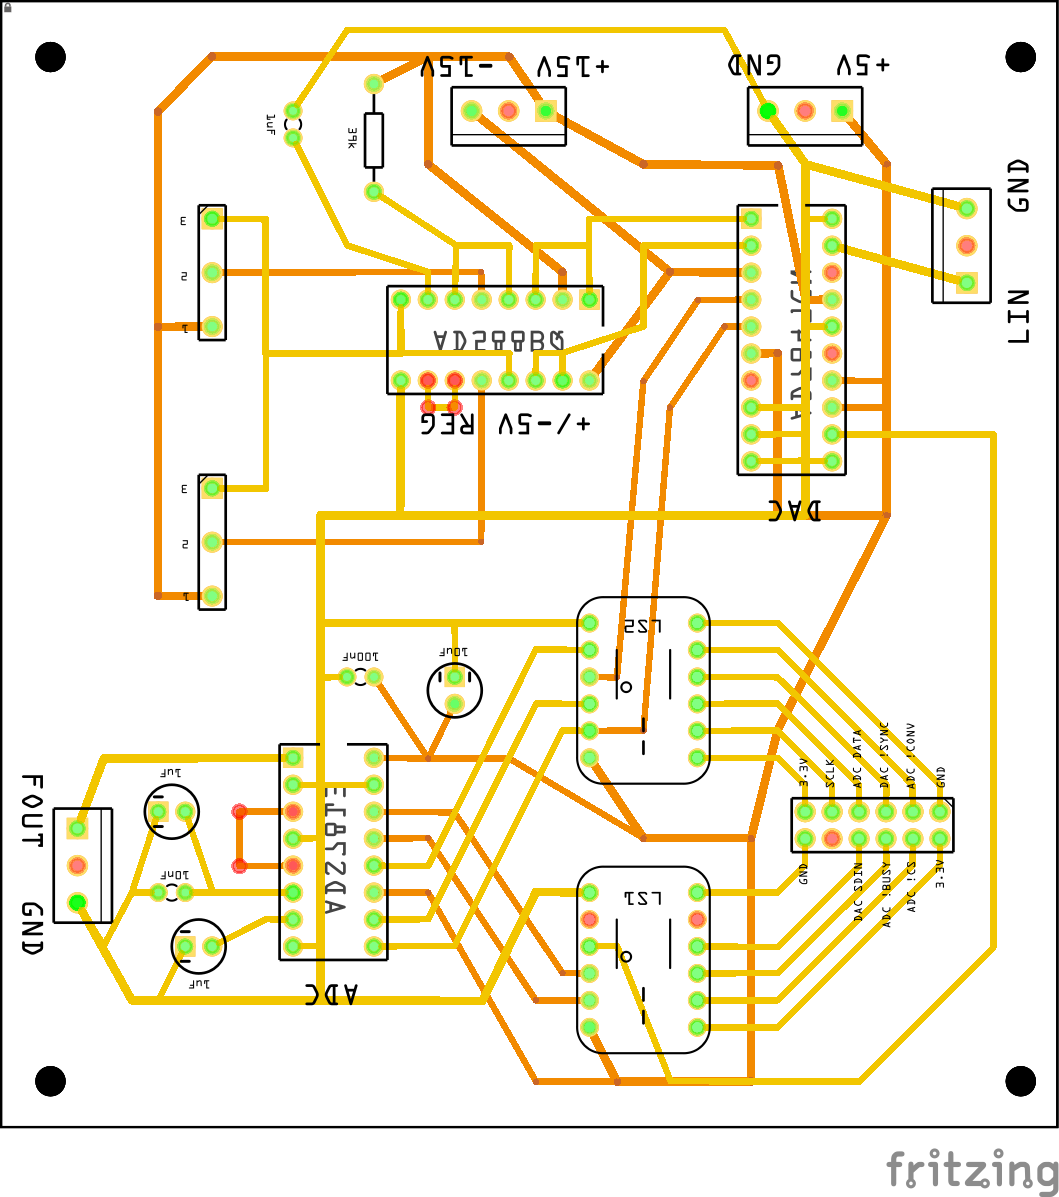
\includegraphics{../ReactiveMotor_Annex_pcb}
	\caption{Reactive motor custom PCB for ADC/DAC interface with Aurora Scientific's motor control system.}
	\label{figAnnex}
\end{figure}

\begin{figure}[!p]
\centering
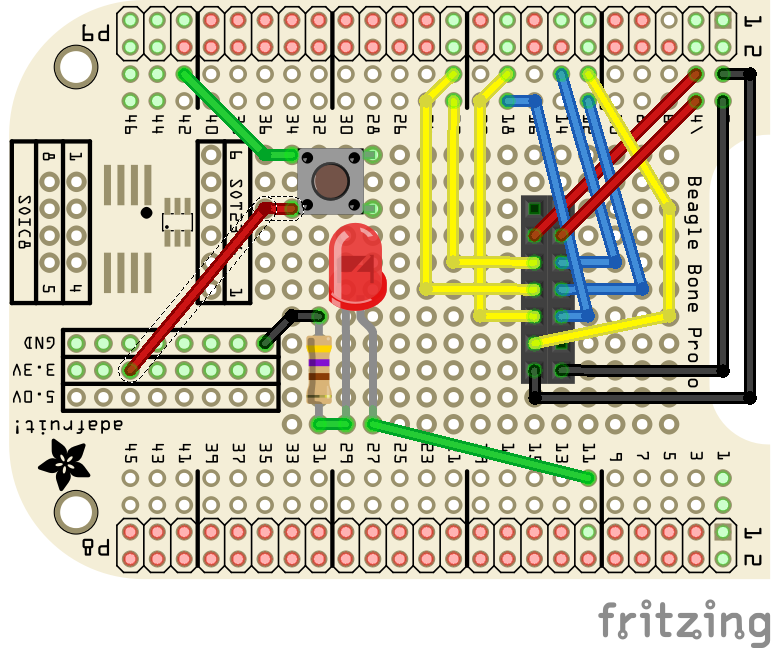
\includegraphics{../ReactiveMotor_Cape_bb}
\caption{Custom BeagleBone cape for BeagleBone-ADC/DAC interface.}
\end{figure}

\section{Room for Improvement}
\begin{itemize}
	\item Cleaner power source
	\item Redesign PCB to reduce electrical noise
	\item A digital filter with more logic and less duct-tape-and-spit
	\item Take advantage of BeagleBone's PRU for higher control loop frequency. Aurora's delay will still be a limiting factor; read/write to motor takes approximately 3 ms. Also, collaborators may have a tougher time reading and editing in the PRU's assembly language.
	\item Switch to a non-Aurora system that doesn't require this Rube Goldberg device.
\end{itemize}
	
\newpage
\part{Cheat Sheet}

SSH connection
\begin{itemize}
	\item BeagleBone's IP address: \texttt{192.168.7.2}
	\item login name: \texttt{root}
\end{itemize}

BeagleBone terminal commands
\begin{itemize}
	\item list current folder's contents: \texttt{ls}
	\item copy code: \texttt{cp <original\_file\_name.cpp> <new\_copy\_name.cpp>}
	\item edit code: \texttt{nano <file\_name.cpp>}
	\begin{itemize}
		\item scroll: arrow keys
		\item select a section of code: hold \texttt{SHIFT} while scrolling with arrow keys
		\item copy: mouse right-click menu
		\item paste: mouse right-click menu
		\item save: \texttt{CTRL+o}
		\item exit: \texttt{CTRL+x}
	\end{itemize}
	\item compile code: \texttt{g++ <file\_name.cpp> GPIO.cpp -o <file\_name.o> -pthread}
	\item execute code: \texttt{./<file\_name.o>}
	\item safely disconnect BeagleBone: \texttt{poweroff}
	\item close terminal window: \texttt{exit}
\end{itemize}
Plug your own file names in for terms marked with triangular brackets \texttt{<>}. Do not type the brackets.


\end{document}